\section{\ce{[Cd(dca)_2(4-methoxypyridine)_2]_n}}
\subsection{Synthesis}
0.52 g \ce{CdSO_4* 8/3 H_2O} (2 mmol), 0.36 g Na-dca (4 mmol) and 0.44 g 4-methoxypyridine (4 mmol) were dissolved in 40 mL distill. \ce{H2O}. The mixture was stirred for 140 minutes (at 70$^\circ$C). After the removal of solid compounds, the colourless solution was stirred at the same temperature for 20 minutes. Thereafter the solution was allowed to cool down to RT. After one day white crystals were obtained. Anal. Calculated for \ce{C_{16}H_{14}CdN_{8}O_{2}} (462.76 g/mol) : 41.53\% C; 3.05\% H; 24.21\% N; Found: 41.55 \% C; 3.11\% H; 24.25 \% N; IR (ATR, cm$^{-1}$): 2295 (m), 2227 (m), 2171 (s), 1607 (s), 1566 (m), 1434 (s), 1348 (s), 1302 (s), 1206 (s), 1027 (vs), 933 (w), 813 (s), 711 (w), 675 (m), 569 (w), 521 (s), 461 (m)

\begin{figure}[htpb!]
\centering
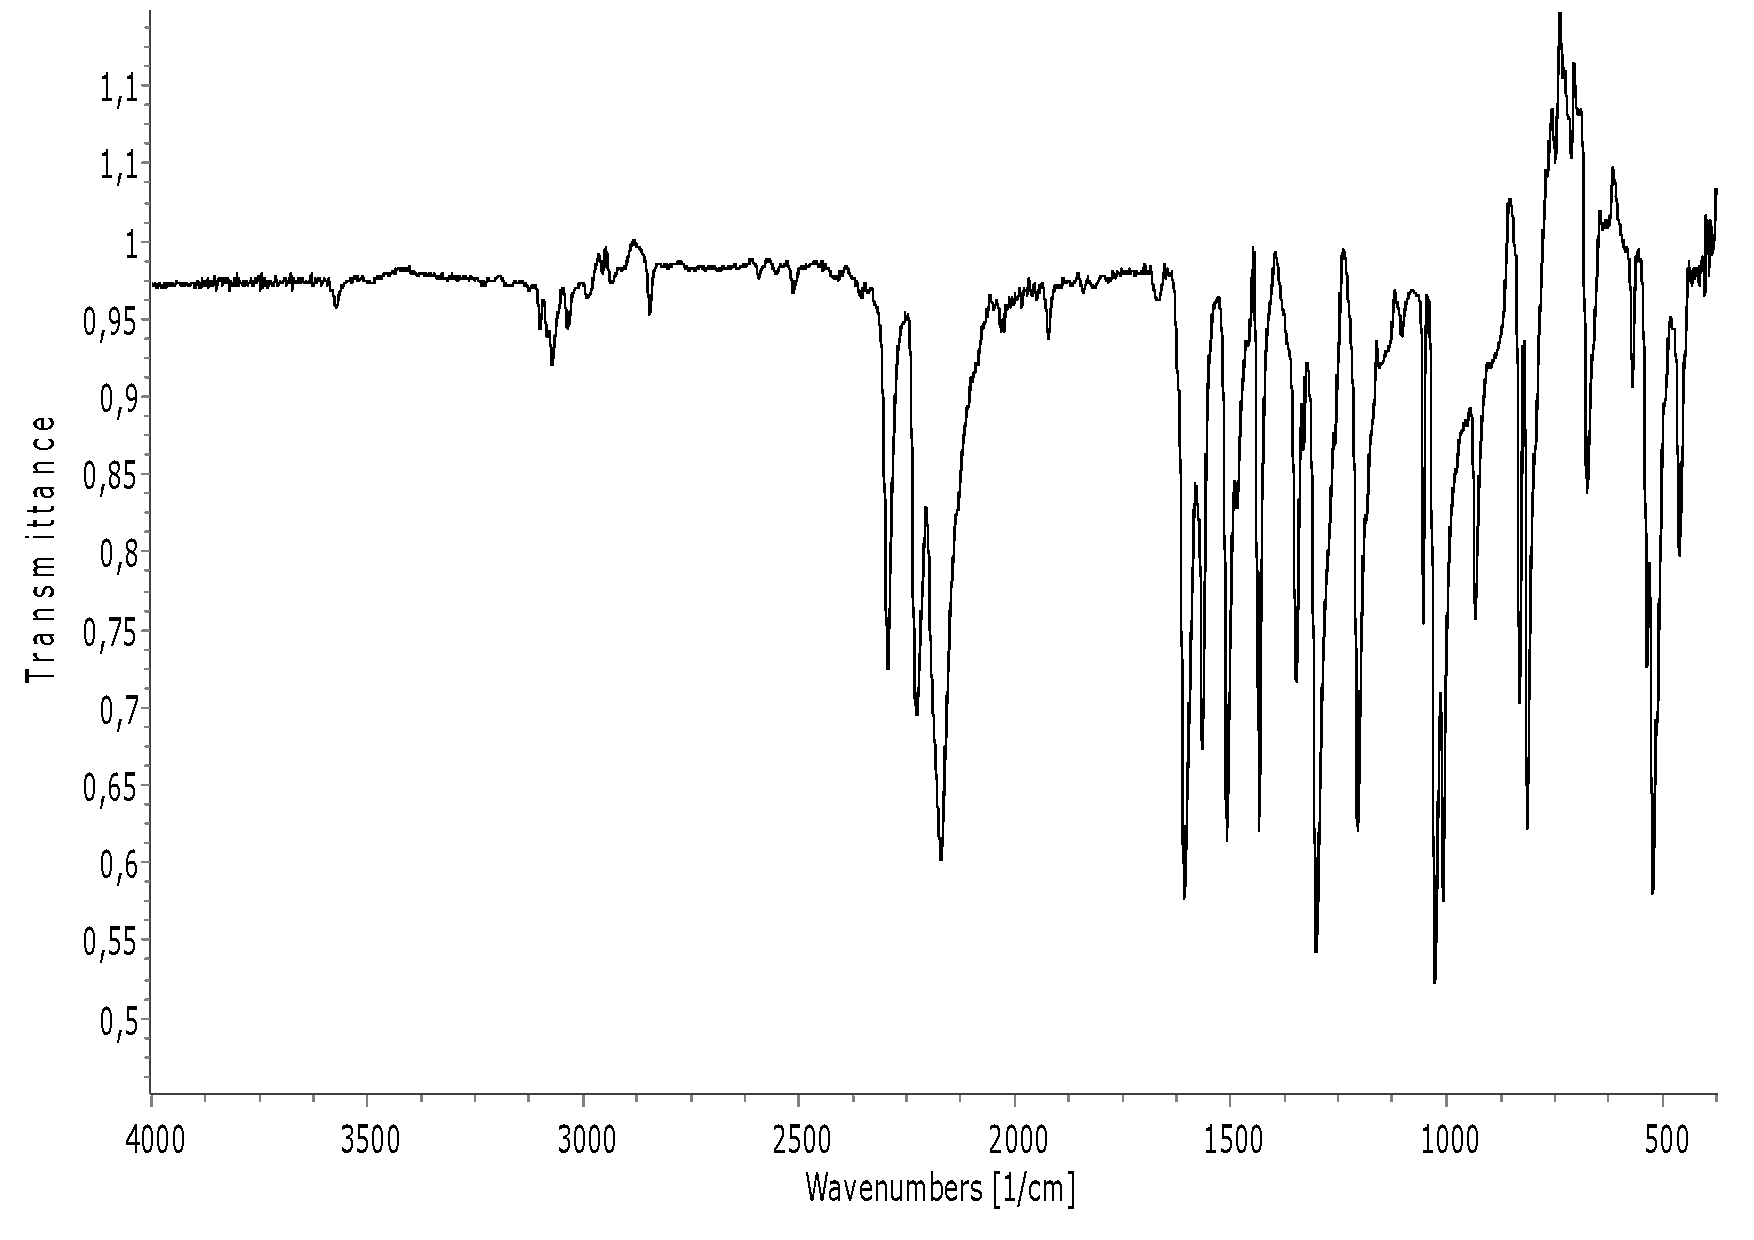
\includegraphics[width=1\textwidth]{figures/CdD4MOP-IR_1.pdf}
\caption{IR spectrum of \ce{[Cd(dca)_2(4-MeOpy)_2]_n}}
\end{figure}


\newpage
\subsection{Structural characterization}
 Selected bond parameters of \ce{[Cd(dca)_2(4-MeOpy)_2]_n} are summarized in table \ref{batab:CdD4MOP}, A perspective view of a section of the polymeric chain is given in fig. \ref{fig:CdD4MOP_pv} and a packing view in fig. \ref{fig:CdD4MOP_packv}.  The Co(1) center (located on an inversion center) is coordinated by a pyridine N donor atom for each of two 4-methoxypyridine molecules in trans configuration. Four N atoms of dicyanamide anions act in the bis-$\mu$(1,5)-bridging mode to generate polymeric chains of polyhedra. These atomes are oriented along the b-axis of the triclinic unit cell. The \ce{CdN_6} polyhedron forms an almost regular octahedron, with Cd-N bond distances varying from 2.302(3) to 2.344(4) \AA, and maximum deviation 3.34$^\circ$ of the N-Cd-N bond angles from 90 or 180$^\circ$. The dicyanamide bridges have the following bond parameters: Cd-N-C: 161.7(4) and 155.7(4)$^\circ$; N-C-N: 174.1(5) and 176.0(5)$^\circ$; C-N-C: 118.9(3)$^\circ$; C-N(nitril) 1.150(6) and 1.159(6) \AA; C-N(amide): 1.313(6) and 1.313(6) \AA. The intra-chain Cd\ce{***}Cd distance of 7.5491(9)\AA  is longer than the shortest inter-chain metal\ce{***}metal separation of 7.1028(8) \AA. 

\renewcommand{\arraystretch}{1.5}
\begin{table}[htpb!]
\centering
\captionabove{Selected bond lengths (\AA) and angles ($^\circ$) for \ce{[Cd(dca)_2(4-MeOpy)_2]_n}; Symmetry codes: (a) 2-x,2-y, -z; (b) 2-x, 1-y, -z; (c) x, 1+y, z; (d) x, -1+y, z; (e) 2-x, 3-y, -z; (f) 2-x, -y, -z.}
\begin{tabular}{|l|l|l|l|}
\hline
Cd(1)-N(1a) & 2.302(3) & Cd(1)-N(4b) & 2.344(4)\\
\hline
Cd(1)-N(2a) & 2.342(4) & N(3)-C(7) & 1.313(6)\\
\hline
N(2)-C(7) & 1.150(6) & N(3)-C(8) & 1.313(6)\\
\hline
N(4)-C(8) & 1.159(6) &  & \\
\hline
\hline
N(1)-Cd(1)-N(2a) & 91.32(13) & N(1)-Cd(1)-N(4b) & 90.58(13)\\
\hline
N(4c)-Cd(1)-N(2a) & 93.34(11) & N(2)-Cd(1)-N(2a) & 180.0\\
\hline
Cd(1)-N(2)-C(7) & 161.7(4) & N(2)-C(7)-N(3) & 174.1(5)\\
\hline
Cd(1b)-N(4)-C(8) & 155.7(4) & N(4)-C(8)-N(3) & 176.0(5)\\
\hline
C(7)-N(3)-C(8) & 118.9(3) &  & \\
\hline
\end{tabular}

\label{batab:CdD4MOP}
\end{table}

\begin{figure}[!htpb]
\centering
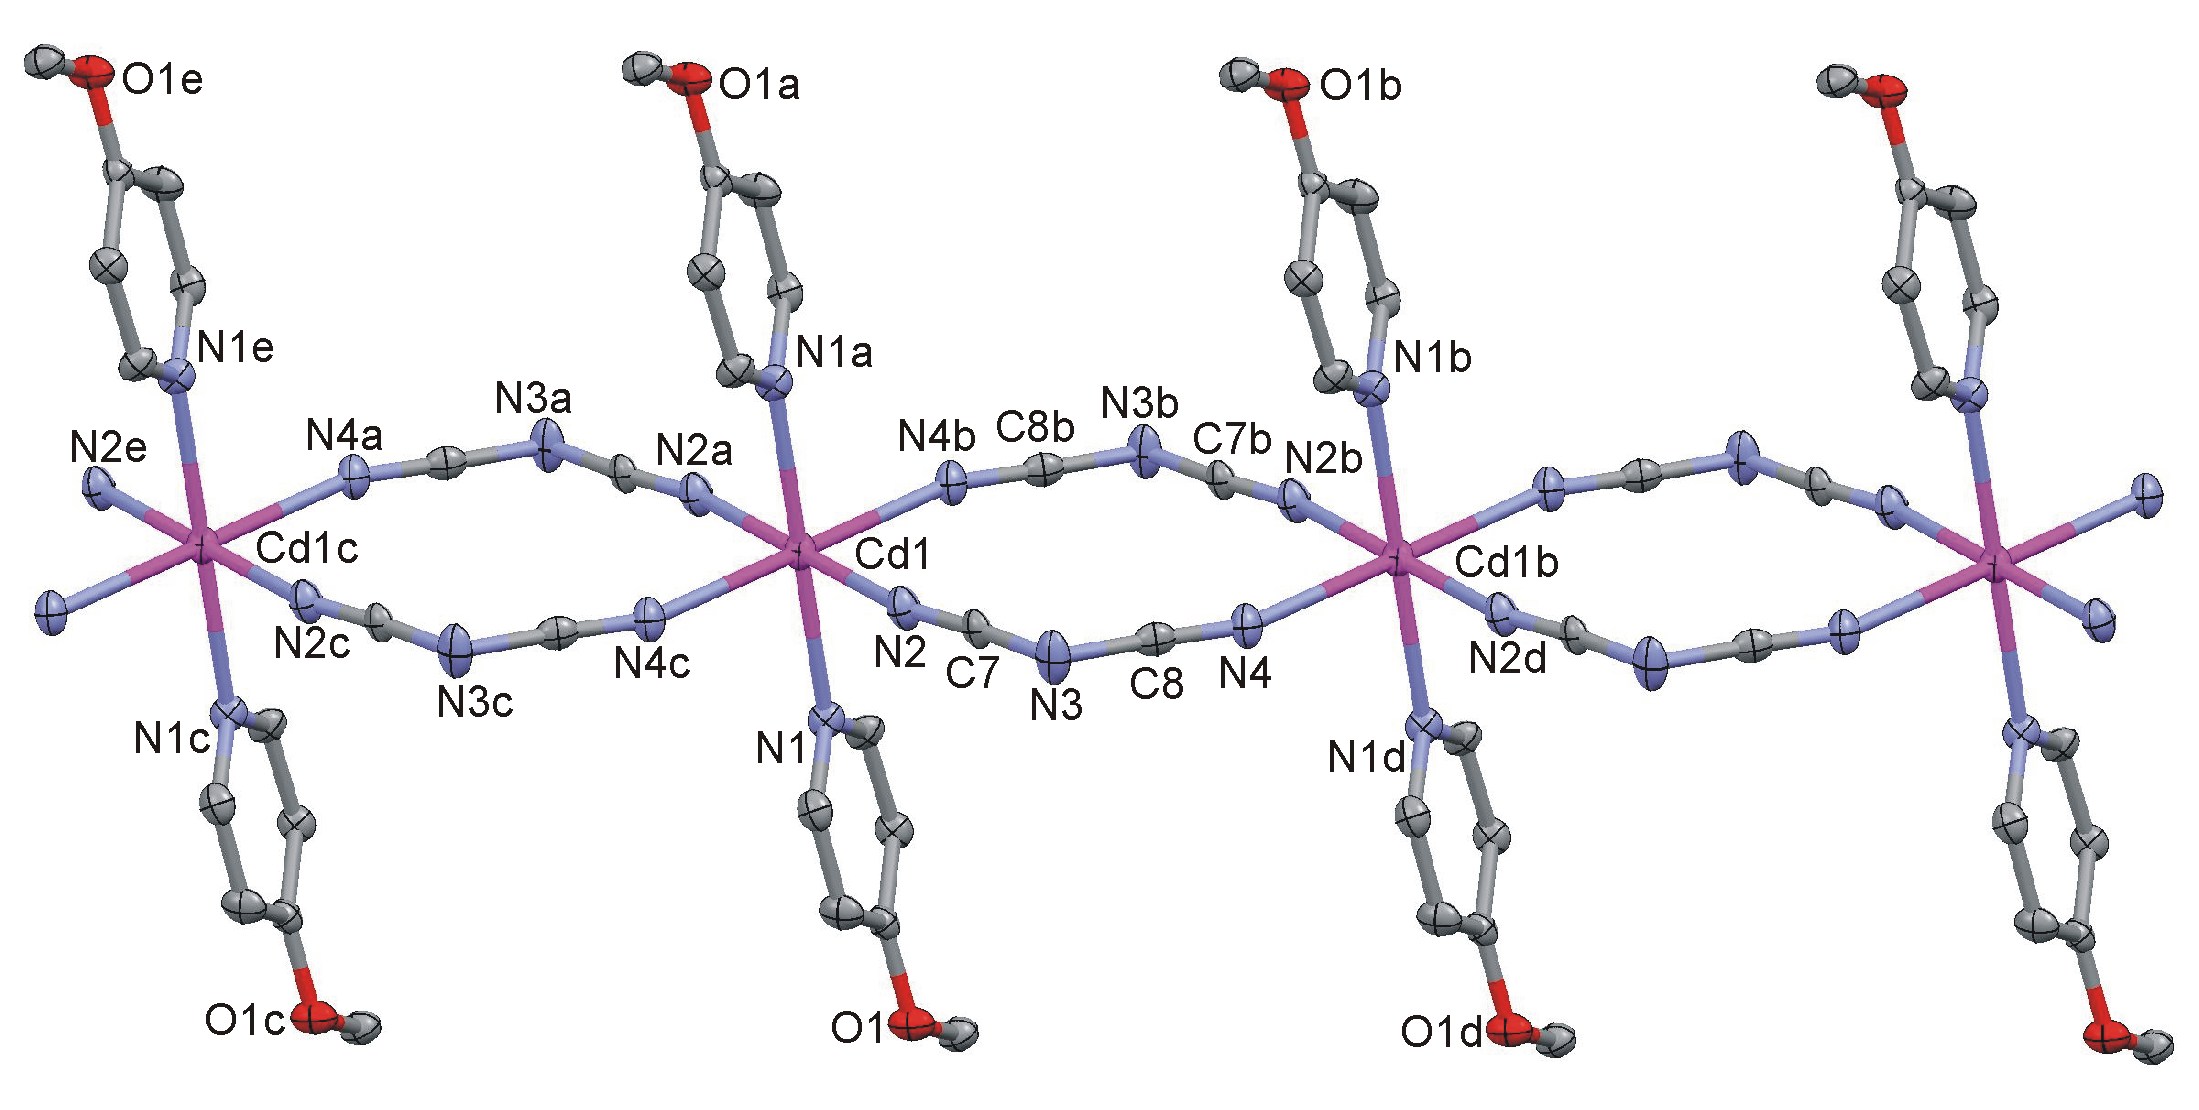
\includegraphics[width=1\textwidth]{figures/cddca4mop_FIGm11.png}
\caption[Perspective view of \ce{[Cd(dca)_2(4-MeOpy)_2]_n}]{Perspective view of a section of the polymeric chain of  \ce{[Cd(dca)_2(4-MeOpy)_2]_n} together with the atom numbering scheme. Symmetry codes: (a) 2-x,2-y,-z; (b) 2-x,1-y,-z; (c) x,1+y,z; (d) x,-1+y,z; (e) 2-x,3-y,-z; (f) 2-x,-y,-z.}
\label{fig:CdD4MOP_pv}
\vspace{\floatsep}
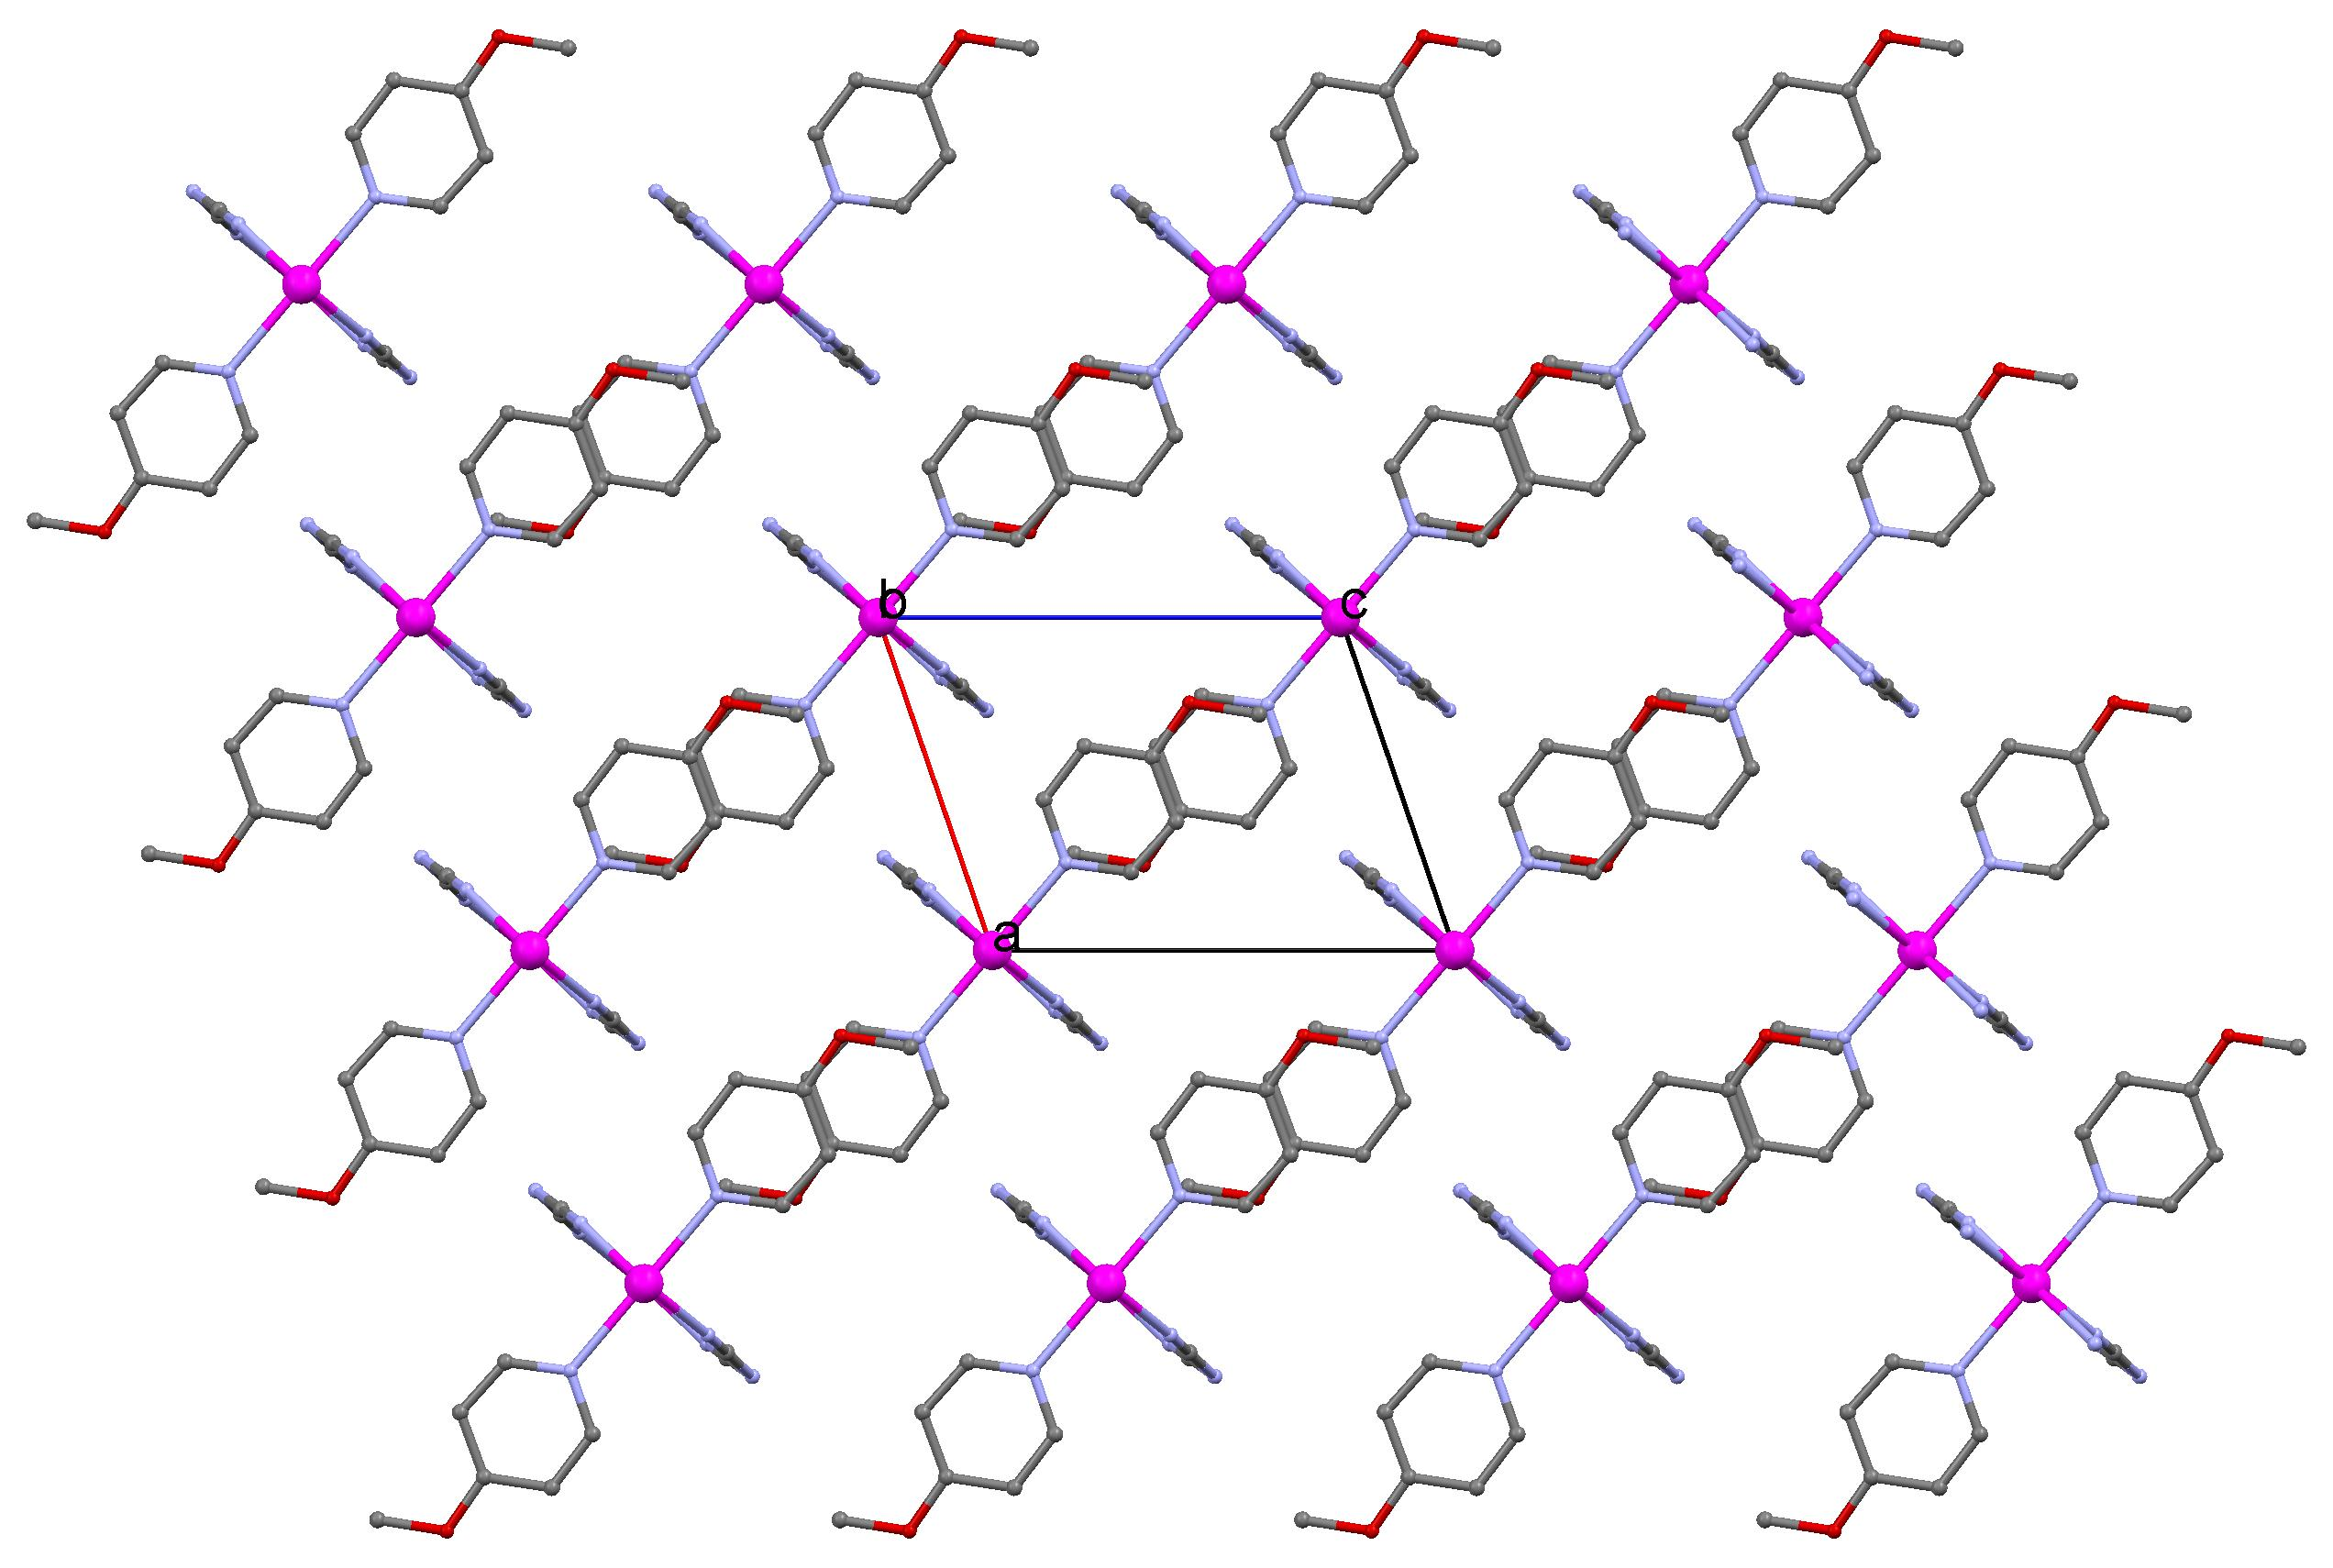
\includegraphics[width=1\textwidth]{figures/cddca4mop_CB.png}
\caption{Packing plot of \ce{[Cd(dca)_2(4-MeOpy)_2]_n}.}
\label{fig:CdD4MOP_packv}
\end{figure}




\begin{table}
\centering
\captionabove{Crystallographic data and processing parameter of \ce{[Cd(dca)_2(4-MeOpy)_2]_n}}
\begin{tabular}{ | l |  l | }
\hline
Empirical formula & \ce{C_{16}H_{14}CdN_{8}O_{2}}\\
\hline
Formula mass & 462.76\\
\hline
System & triclinic\\
\hline
Space group & P-1\\
\hline
a ({\AA}) & 7.1028(8)\\
\hline
b ({\AA}) & 7.5491(8)\\
\hline
c ({\AA}) & 9.8206(11)\\
\hline
$\alpha$ ($^\circ$) & 71.234(5)\\
\hline
$\beta$ ($^\circ$) & 70.587(5)\\
\hline
$\gamma$ ($^\circ$) & 85.267(5)\\
\hline
V (\AA$^{3}) $  & 470.06(9)\\
\hline
Z & 1\\
\hline
T (K) & 100(2)\\
\hline
$\mu$ (mm$^{-1}$) & 1.190\\
\hline
 D$_{calc}$ (Mg/m$^{3}$) & 1.635\\
\hline
Crystal size (mm) & 0.22 x 0.14 x 0.09\\
\hline
$\theta$ max ($^\circ$) & 27.00\\
\hline
Data collected & 2003\\
\hline
Unique refl./ R$_{int}$ & 2003 / ----\\
\hline
Parameters & 126\\
\hline
Goodness-of-Fit on F$^{2}$ & 1.040\\
\hline
R1 / wR2 (all data) & 0.0383 /0.0836\\
\hline
Residual extrema (e/\AA$^{3}$) & 0.95 /-1.05\\
\hline
\end{tabular}

\label{ptab:CdD4MOP}


\end{table}




